\chapter{Implementacja projektu}

Projekt `Planning poker', to aplikacja webową opartą o platformę Firebase,
która jest napisana przy użyciu bibliotek React.js w programie visual studio code.
Aby zachować porządek i możliwość późniejszego rozwoju aplikacji o nowe komponenty,
koniecznym jest stworzenie uporządkowanej struktury plików zawartych w projekcie.
~rys.\ref{rys:projekt}
\begin{figure}
	\centering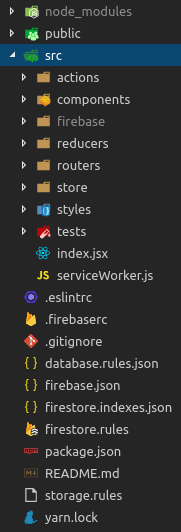
\includegraphics[width=.2\textwidth]{img/projekt}
	\caption{Struktura projektu}\label{rys:projekt}% Źródło rysunku i etykieta przez którą odwołujemy się do rysunku.
\end{figure}
Folderem zawierającym wszystkie podfoldery oraz pliki jest folder `scrumpoker' (jest to druga wersja aplikacji).
Pliki takie jak `storage.rules' czy `.firebaesrc' powstały automatycznie w procesie konfiguracji usługi firebase.
Plik `package.json' zabiera całą konfigurację projetku stworzonego dzięki narzędziu `create-react-app'.
Folder `node modules' zawiera zawiera zależności, niezbędne do uruchomienia aplikacji.
    Folder src zawiera cały kod aplikacji. Jest on najważniejszy w całym projekcie.
Głównym plikiem projektu jest `index.jsx'. To w tym pliku renderowana jest cała aplikacja.
Aby uruchomić program niezbędny jest też backend w postaci utworzonego i skonfigurowanego projektu firebase.
Konfiguracje należy umieścić w pliku `src/firebase/firebase.jsx'. Listing:
~\ref{listing:firebaseConfig} 

\begin{listing}
	\begin{minted}{c}
import * as firebase from 'firebase';

var config = {
    apiKey: "<API_KEY>",
    authDomain: "<PROJECT_ID>.firebaseapp.com",
    databaseURL: "https://<DATABASE_NAME>.firebaseio.com",
    projectId: "<PROJECT_ID>",
    storageBucket: "<BUCKET>.appspot.com",
    messagingSenderId: "<SENDER_ID>",
  };

firebase.initializeApp(config);

const database = firebase.firestore();
const settings = { timestampsInSnapshots: true};
database.settings(settings);
export { firebase, database as default };
	\end{minted}
	\caption{Konfiguracja firebase} \label{listing:firebaseConfig}
\end{listing}

Aplikacaja wszelkie dane, oprócz danych na temat stanu gry pobiera z serwisu `Github',
dzieki biliotece `octokit/rest'.  W każdym komponencie, wymagającym danych z tego serwisu,
uruchamiane są metody, które ładują niezbędne dane do stanu komponentu.
Jako, że wszelkie gry tworzone w aplikacji dotyczą projektów prowadzonych na githubie,
użytkownik aby skorzystać z aplikacji musi posiadać konto na githubie oraz co naimniej jeden projekt
na tym serwisie. Biorąc pod uwagę, że w trakcie planning pokera oceniane są historyjki z backlogu,
użytkownik musi mieć jakieś gotowe historyjki w githubie. Aby to zrobić musi utworzyć w projekcie,
elementy zwane `issues', które w tym momencie traktowane są jako historyjki.
Co za tym idzie użytkownik musi się zalogować przez serwis Github co pokazuje poniższy rysunek.
~\ref{rys:login} 

\begin{figure}
	\centering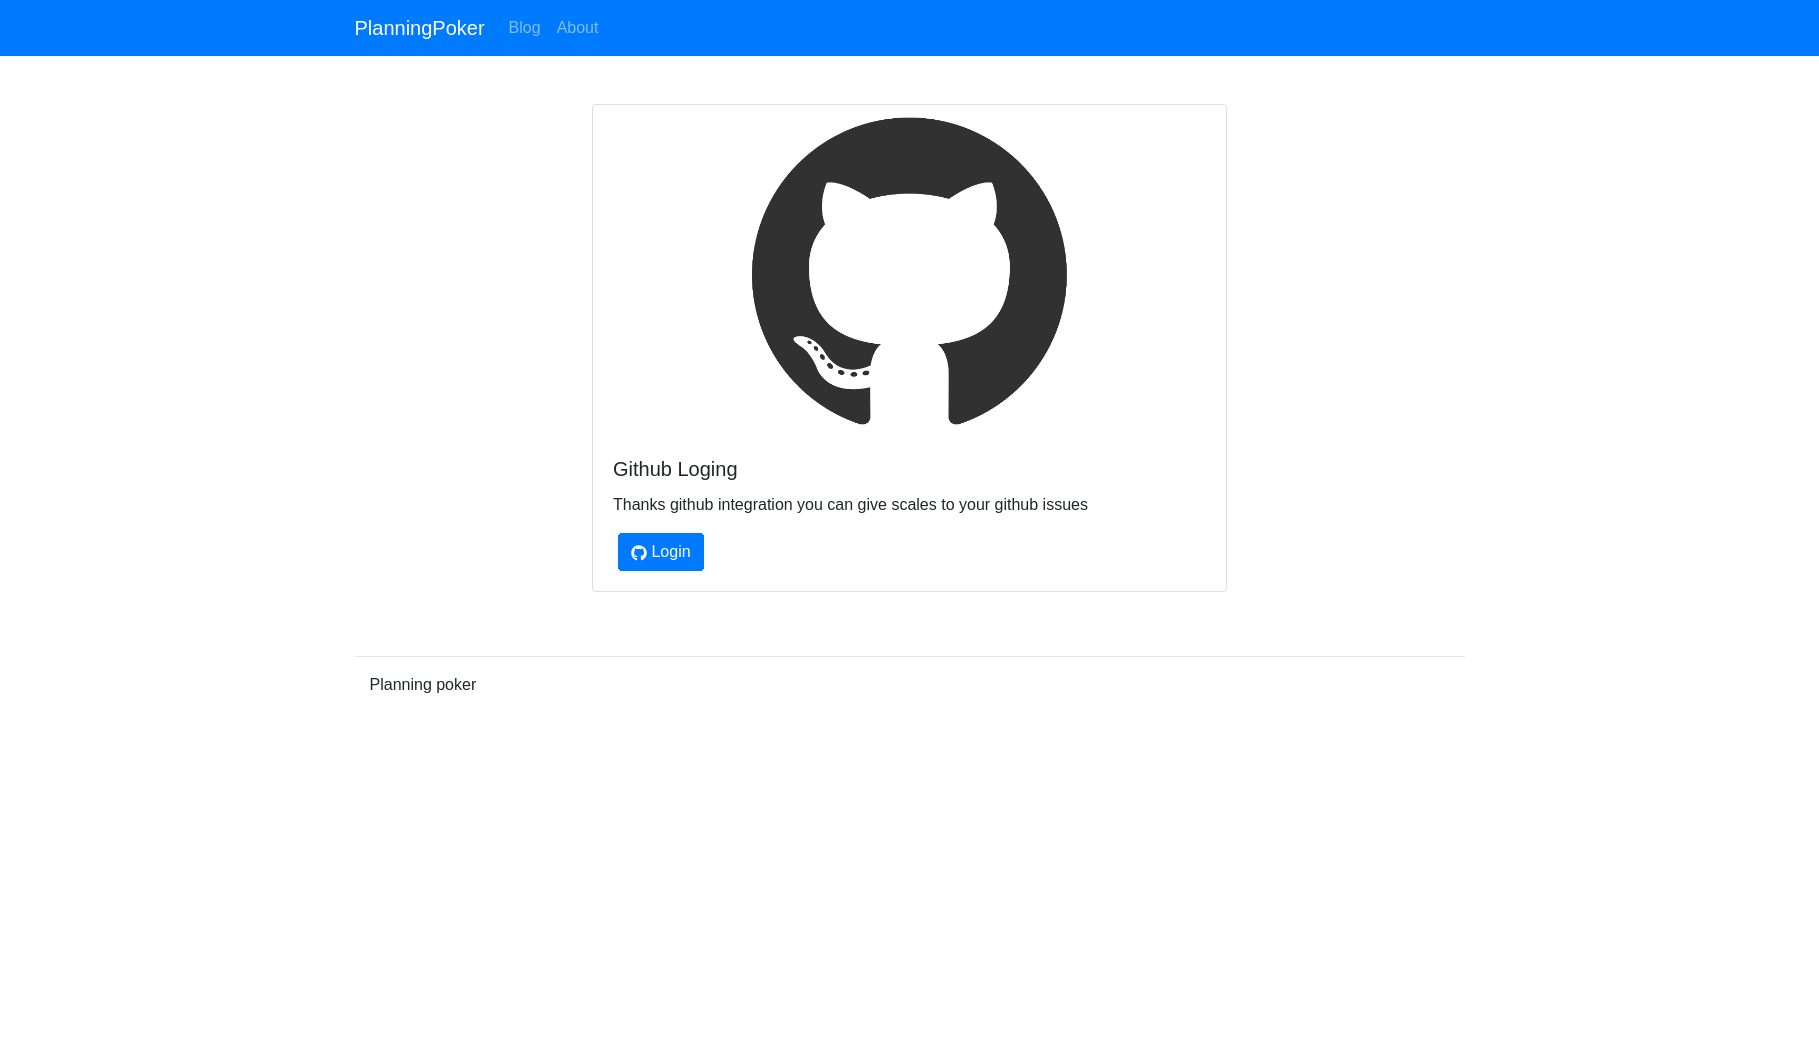
\includegraphics[width=.7\textwidth]{img/GitLogin}
	\caption{Strona logowania}\label{rys:login}% Źródło rysunku i etykieta przez którą odwołujemy się do rysunku.
\end{figure}

\section{Tworzenie gry}
Aby utworzyć grę, najpierw należy wybrać projekt, której gra będzie dotyczyła.
W aplikacji projektami są repozytoria. Rysunek: 
~\ref{rys:projekty}
\begin{figure}
	\centering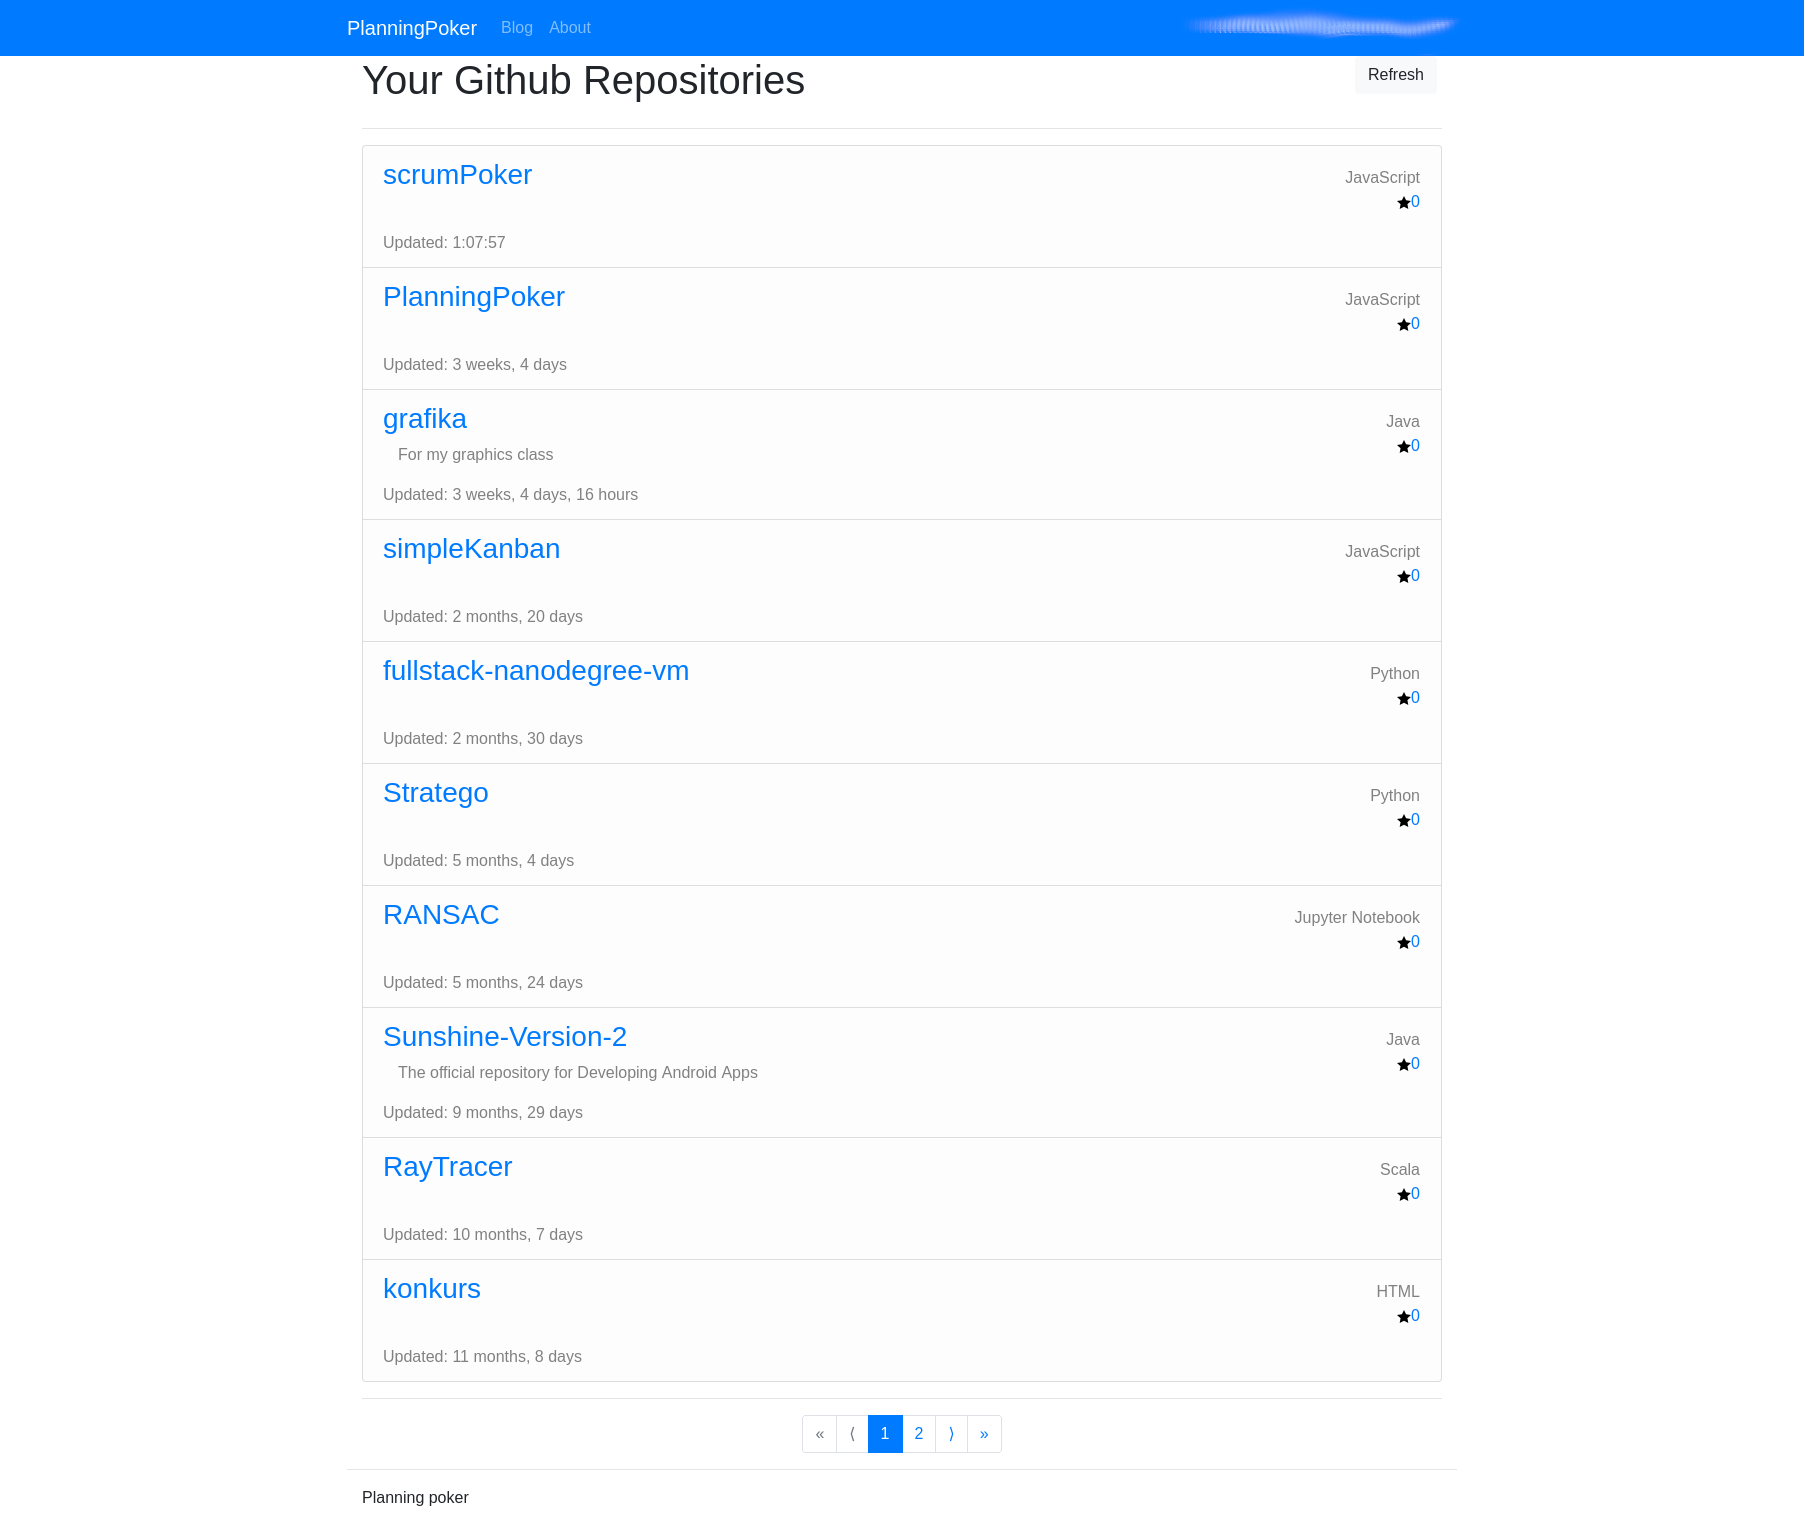
\includegraphics[width=.7\textwidth]{img/repositories}
	\caption{Ekran wyboru projektu}\label{rys:projekty}% Źródło rysunku i etykieta przez którą odwołujemy się do rysunku.
\end{figure}
Można więc wywnioskować, że grupą docelową aplikacji, są użytkownicy githuba, czyli programiści.
Tak właśnie jest, gdyż jako członek tej grupy odczułem brak aplikacji, która byłaby z tym narzędziem zintegrowana.
Podczas przeglądania projektów na githubie, zauważyłem, że użytkownicy czy też programiści,
wszelkie problemy czy też propozycje nowych funkcjonalności aplikacji są umieszczane w sekcji issues projektu.
Stwierdziłem wówczas, iż aplikacja, która ocenia istniejące problemy lub proponowane cechy, które są dostępne,
w już sprawdzonym narzędziu i eksportuje oceny do githuba w postaci etykiet będzie dobrym pomysłem.
Aby stworzyć grę należy stworzyć listę zwaną backlogiem, która jest listą `issues'.
Tworzy się ją w panelu repozytorium w sekcji `Issues' rys.
~\ref{rys:issues} 
\begin{figure}
	\centering\includegraphics[width=.7\textwidth]{img/issues}
	\caption{Ekran projektu}\label{rys:issues}% Źródło rysunku i etykieta przez którą odwołujemy się do rysunku.
\end{figure}
\begin{figure}
	\centering\includegraphics[width=.7\textwidth]{img/Formularz}
	\caption{Formularz tworzenia gry}\label{rys:form}% Źródło rysunku i etykieta przez którą odwołujemy się do rysunku.
\end{figure}
Dzięki odpowiednim filtrom można przefiltrować elementy po etykietach, autorze, czy po kamieniach milowych.
Aby stworzyć listę należy wybrać odpowiednie zagadnienia,
klikając lewy przycisk myszy, czy też zaznaczając stronę za pomocą przycisku `Check page'.
Po wybraniu odpowiednich elementów i naciśnięciu przycisku `Create List' pokazywane jest okno potwierdzenia,
które pokazuje wybrane elementy oraz pole do wpisania nazwy listy.
Po potwierdzeniu wyboru oraz wpisaniu nazwy listy, jest tworzona lista, zawierająca identyfikatory wybranych `issues'.
Jak zostało już wcześniej wspomniane, niezbędnym elementem każej gry jest backlog.
Tym backlogiem dla każdej gry będzie lista, którą właścicel gry tworzy przed każdym stworzeniem gry.
Ta lista będzie później dostępna w formularzu tworzenia gry,
dzięki czemu będzie można ją wybrać przy jej tworzeniu.
W trakcie tworzenia gry, możemy określić jej nazwę i opis ale także parametry, które będą miały wpływ na grę.
Oczywiście, będziemy mogli wybrać skalę estymacji gry, ale także podać prędkość naszego zespołu,
zdecydować czy inni gracze będą tą prędkość widzieć.
Możemy także zdecydować czy my jako twórca gry również będziemy głosować.
Inną ważną kwestią jest to, czy karty powinny być odkrywane, kiedy każdy zagłosował
oraz czy pozwolić graczom zmienić swoją ocenę po pokazaniu przez wszystkich kart.
Aplikacja może również obliczać wynik punktowy historyjki po zakończonym głosowaniu automatycznie,
robi to za pomocą średniej ważonej, kóra później jest zamieniana na najbliższą jej ocenę w skali estymacji.
Na końcu oczywiście należy wybrać backlog w postaci odpowiedniej listy, tu należy zaznaczyć,
że jeżeli w projekcie nie będzie stworzonej żadnej listy, to nie będzie można stworzyć gry.
Pewne ustawienia gry można zmienić po jej utworzeniu.
Każda historyjka w grze jest oczywiście przechowywana w bazie w postaci identyfikatora.
Formularz tworzenia gry jest pokazany na rysunku: 
~\ref{rys:form} 

\section{Rozgrywka}

Aby rozgrywka w planning pokera była możliwa,
konieczna jest asynchroniczna komunikajca z serwerem.
Wszelkie akcje podczas gry są synchronizowane za pomocą `Firebase',
a dzięki odpowiednim słuchaczom aplikacja reaguje na wszelkie zmiany w stanie gry.
Aby gra się odbyła potrzebny jest nie tylko backlog, ale także i gracze.
Gracz jest dodawany do gry poprzez udostępnianie innym użytkownikom odnośnika do gry w postaci jej adresu.
Jeżeli gracz wejdzie do gry, zostanie poproszony o podanie nazwy,
dzięki której będzie można go odróżnić od innych graczy.
Gracze są dodawani do bazy danych dzięki funkcji usługi firebase nazwanej anonimowe logowanie.
Panel gry pokazuje rysunek:
~\ref{rys:gra}
\begin{figure}
	\centering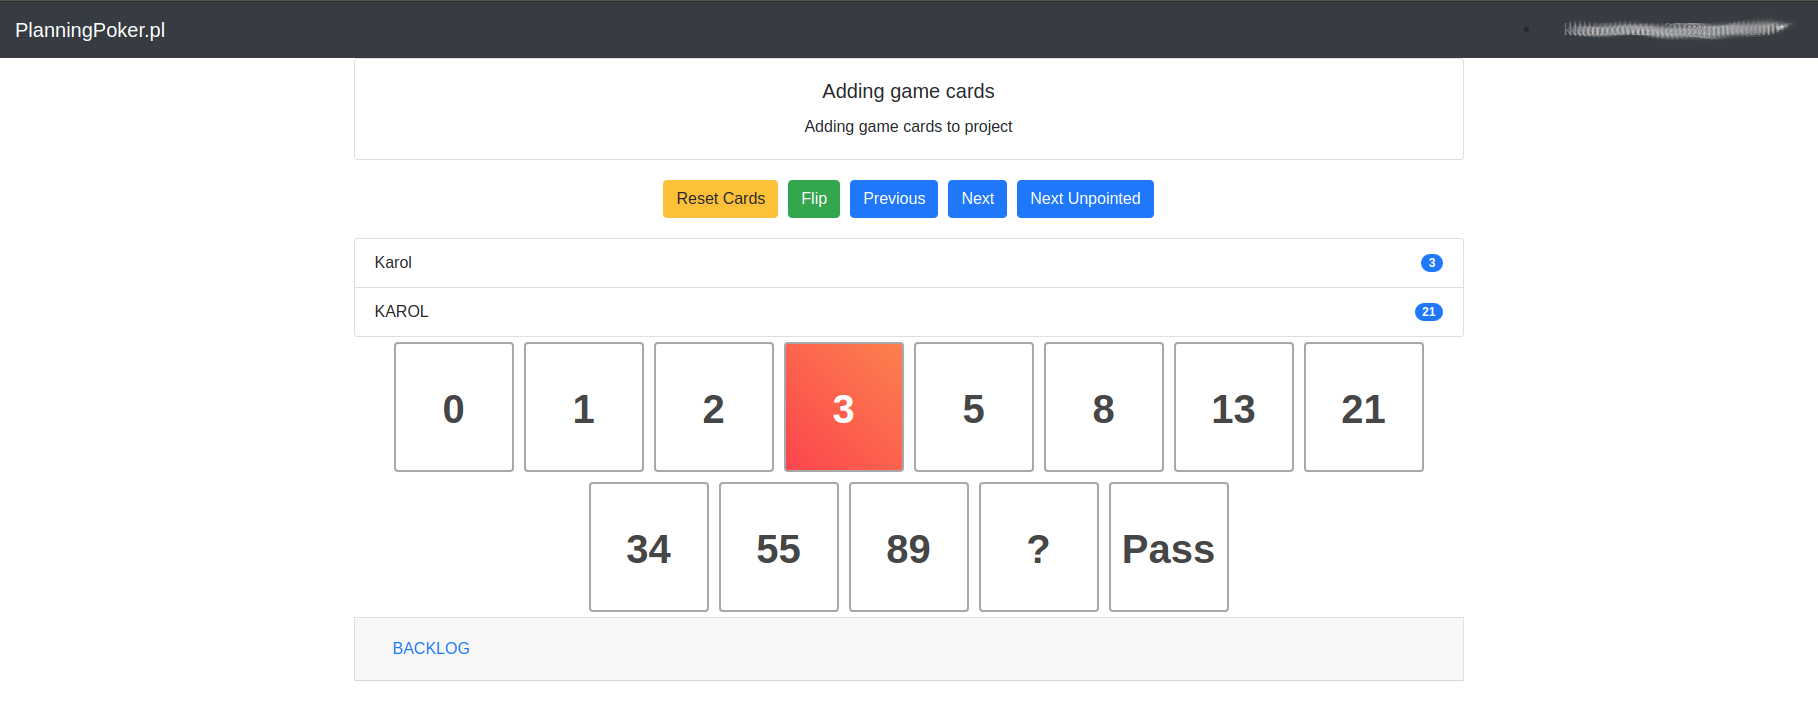
\includegraphics[width=.7\textwidth]{img/gra}
	\caption{Panel gry}\label{rys:gra}% Źródło rysunku i etykieta przez którą odwołujemy się do rysunku.
\end{figure}
Istotnym elementem każdego planning pokera jest komunikacja między graczami,
autor jednak stwierdził,
iż na rynku istnieją już odpowiednie aplikacje do komunikacji,
a firmy produkujące oprogramowanie mają preferowane komunikatory.
A więc przed każdą rozgrywką autor poleca wybrać odpowiedni komunikator do komunikacji w trakcie gry.
Gracze w grze mogą tylko i widocznie głosować,
natomiast to właściciel gry wybiera historyjkę do głosowania, to znaczy że to on narzuca tempo gry.